%# -*- coding: utf-8 -*-
%!TEX encoding = UTF-8 Unicode
%!TEX TS-program = xelatex
% vim:ts=4:sw=4
%
% 以上设定默认使用 XeLaTex 编译,并指定 Unicode 编码,供 TeXShop 自动识别

% Author: Yunhui Fu <yhfudev@gmail.com>
% License: Creative Commons (CC BY 4.0)

\section{\cnt{Preprocessing: PCA and Whitening}{预处理:主成分分析与白化}{}}

\subsection{\cnt{PCA}{主成分分析}{}}

\subsubsection{\cnt{Introduction}{引言}{}}

\cnt{Principal Components Analysis (PCA) is a dimensionality reduction algorithm that can be used to significantly speed up your unsupervised feature learning algorithm. More importantly, understanding PCA will enable us to later implement \emph{whitening}, which is an important pre-processing step for many algorithms.}
    {主成分分析(PCA)是一种能够极大提升无监督特征学习速度的数据降维算法。更重要的是,理解PCA算法,对实现白化算法有很大的帮助,很多算法都先用白化算法作预处理步骤。}
    {}

\cnt{Suppose you are training your algorithm on images. Then the input will be somewhat redundant, because the values of adjacent pixels in an image are highly correlated. Concretely, suppose we are training on $16 \times 16$ grayscale image patches. Then $x \in \Re^{256}$ are 256 dimensional vectors, with one feature $x_j$ corresponding to the intensity of each pixel. Because of the correlation between adjacent pixels, PCA will allow us to approximate the input with a much lower dimensional one, while incurring very little error.}
    {假设你使用图像来训练算法,因为图像中相邻的像素高度相关,输入数据是有一定冗余的。具体来说,假如我们正在训练的 $16 \times 16$ 灰度值图像,记为一个256维向量 $x \in \Re^{256}$,其中特征值 $x_j$ 对应每个像素的亮度值。由于相邻像素间的相关性,PCA算法可以将输入向量转换为一个维数低很多的近似向量,而且误差非常小。}
    {}

\subsubsection{\cnt{Example and Mathematical Background}{实例和数学背景}{}} \label{chp:examplemathbackground}

\cnt{For our running example, we will use a dataset $\{x^{(1)}, x^{(2)}, \ldots, x^{(m)}\}$ with $n=2$ dimensional inputs, so that $x^{(i)} \in \Re^2$. Suppose we want to reduce the data from 2 dimensions to 1. (In practice, we might want to reduce data from 256 to 50 dimensions, say; but using lower dimensional data in our example allows us to visualize the algorithms better.) Here is our dataset:}
    {在我们的实例中,使用的输入数据集表示为 $\{x^{(1)}, x^{(2)}, \ldots, x^{(m)}\}$,维度 $n=2$ 即 $x^{(i)} \in \Re^2$。假设我们想把数据从2维降到1维。(在实际应用中,我们也许需要把数据从256维降到50维;在这里使用低维数据,主要是为了更好地可视化算法的行为)。下图是我们的数据集:}
    {}

\begin{figure}[ht] \centering
  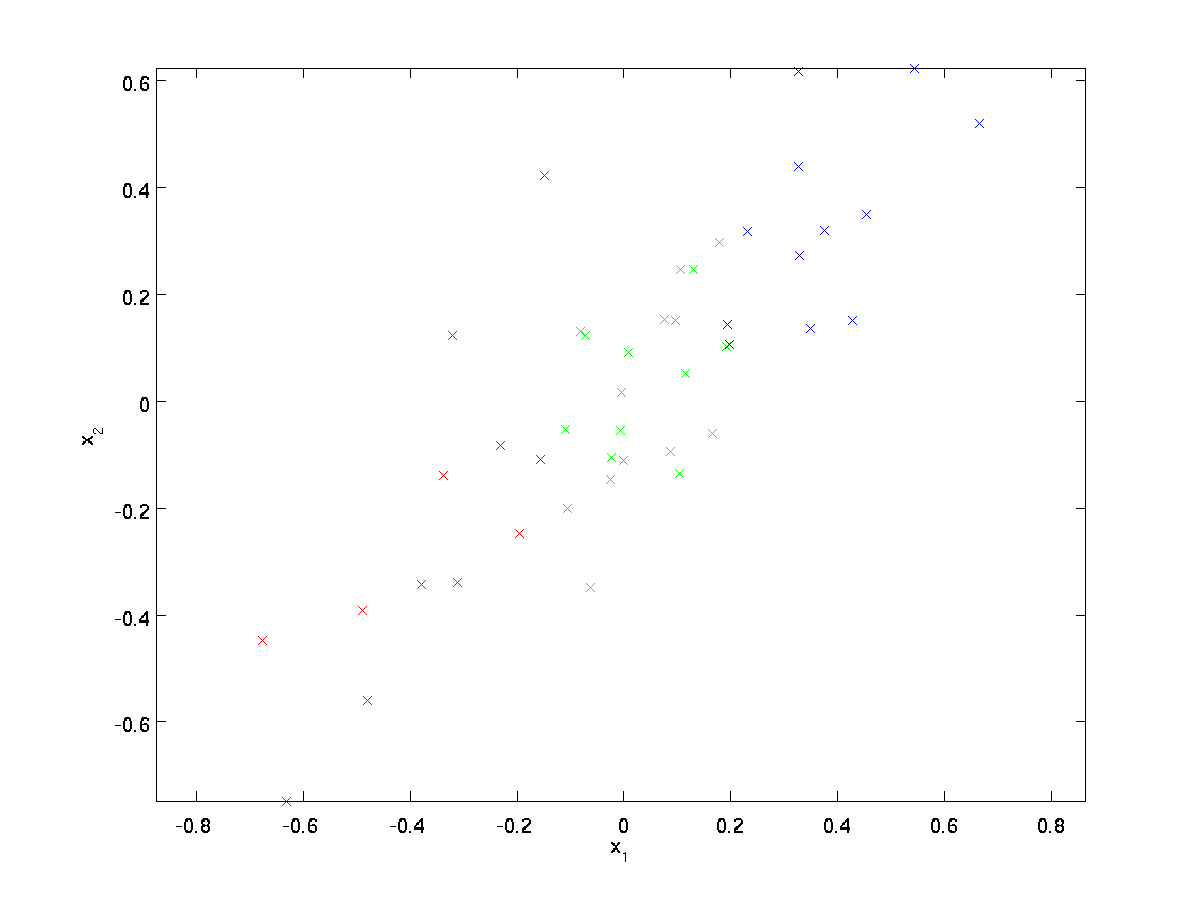
\includegraphics[width=0.8\textwidth]{figures/PCA-rawdata.png}
  %\caption{}\label{fig:step1}
\end{figure}

\cnt{This data has already been pre-processed so that each of the features $x_1$ and $x_2$ have about the same mean (zero) and variance.}
    {这些数据已经进行了预处理,使得每个特征 $x_1$ 和 $x_2$ 具有相同的均值(零)和方差。}
    {}

\cnt{For the purpose of illustration, we have also colored each of the points one of three colors, depending on their $x_1$ value; these colors are not used by the algorithm, and are for illustration only.}
    {为方便展示,根据 $x_1$ 值的大小,我们将每个点分别涂上了三种颜色之一,但该颜色并不用于算法而仅用于图解。}
    {}


\cnt{PCA will find a lower-dimensional subspace onto which to project our data. From visually examining the data, it appears that $u_1$ is the principal direction of variation of the data, and $u_2$ the secondary direction of variation:}
    {PCA算法将寻找一个低维空间来投影我们的数据。从下图中可以看出, $u_1$ 是数据变化的主方向,而 $u_2$ 是次方向。}
    {}

\begin{figure}[ht] \centering
  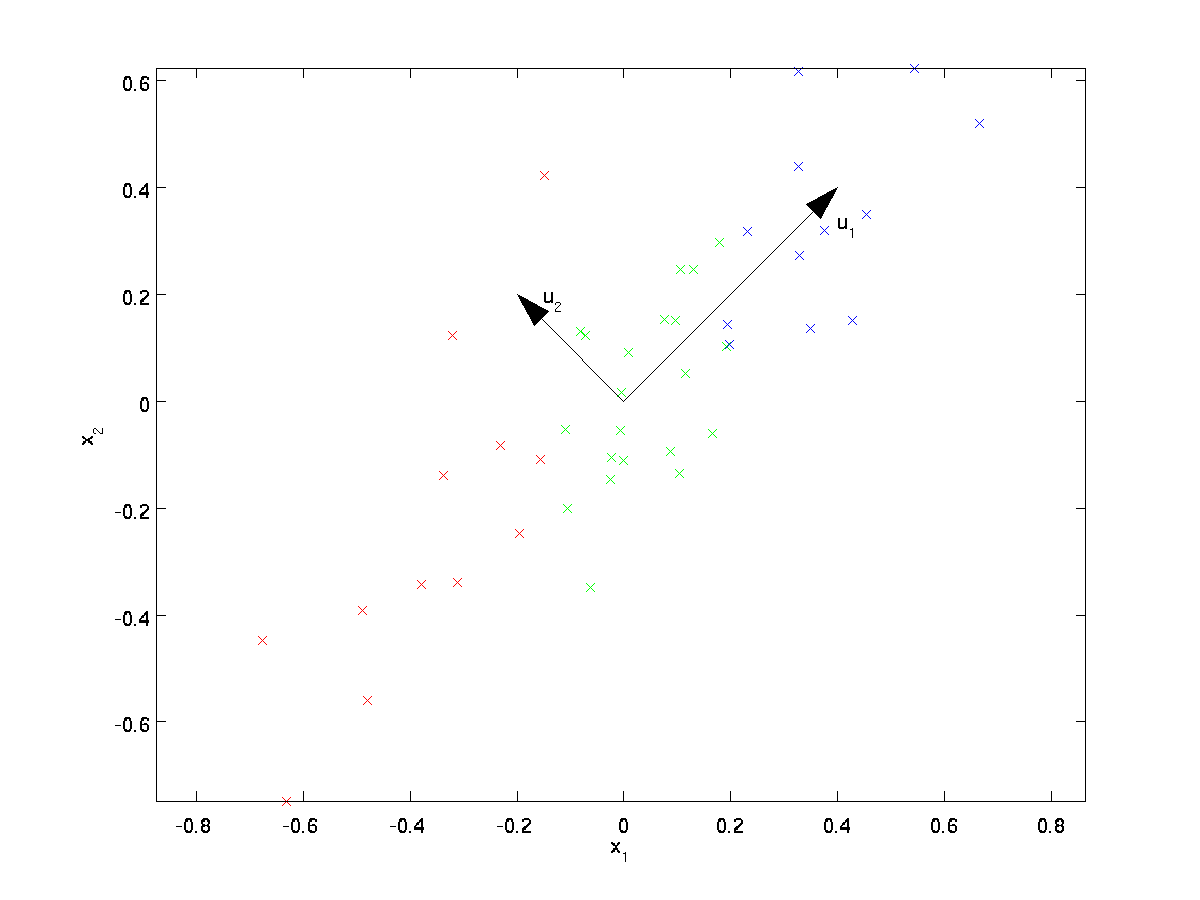
\includegraphics[width=0.8\textwidth]{figures/PCA-u1.png}
  %\caption{}\label{fig:step1}
\end{figure}


\cnt{I.e., the data varies much more in the direction $u_1$ than $u_2$. To more formally find the directions $u_1$ and $u_2$, we first compute the matrix $\Sigma$ as follows:}
    {也就是说,数据在 $u_1$ 方向上的变化要比在 $u_2$ 方向上大。为更形式化地找出方向 $u_1$ 和 $u_2$ ,我们首先计算出矩阵 $\Sigma$,如下所示:}
    {}

\begin{align} \Sigma = \frac{1}{m} \sum_{i=1}^m (x^{(i)})(x^{(i)})^T. \end{align} 

\cnt{If $x$ has zero mean, then $\Sigma$ is exactly the covariance matrix of $x$. (The symbol ``$\Sigma$", pronounced ``Sigma", is the standard notation for denoting the covariance matrix. Unfortunately it looks just like the summation symbol, as in $\sum_{i=1}^n i$; but these are two different things.)}
    {假设 $x$ 的均值为零,那么 $\Sigma$ 就是$x$的协方差矩阵。(符号 $\Sigma$,读``Sigma",是协方差矩阵的标准符号。虽然看起来与求和符号 $\sum_{i=1}^n i$ 比较像,但它们其实是两个不同的概念。)}
    {}


\cnt{It can then be shown that $u_1$ --- the principal direction of variation of the data --- is the top (principal) eigenvector of $\Sigma$, and $u_2$ is the second eigenvector.}
    {可以证明,数据变化的主方向 $u_1$ 就是协方差矩阵 $\Sigma$ 的主特征向量,而 $u_2$ 是次特征向量。}
    {}

\cnt{Note: If you are interested in seeing a more formal mathematical derivation/justification of this result, see the CS229 (Machine Learning) lecture notes on PCA\footnote{Stanford CS229 Machine Learning \url{http://cs229.stanford.edu}} (link at bottom of this page). You won't need to do so to follow along this course, however.}
    {注:如果你对如何得到这个结果的具体数学推导过程感兴趣,可以参看CS229(机器学习)PCA部分的课件\footnote{Stanford CS229 Machine Learning \url{http://cs229.stanford.edu}}(链接在本页底部)。但如果仅仅是想跟上本课,可以不必如此。}
    {}


\cnt{You can use standard numerical linear algebra software to find these eigenvectors (see Implementation Notes). Concretely, let us compute the eigenvectors of $\Sigma$, and stack the eigenvectors in columns to form the matrix \texttt{U}:}
    {你可以通过标准的数值线性代数运算软件求得特征向量(见实现说明).我们先计算出协方差矩阵$\Sigma$的特征向量,按列排放,而组成矩阵\texttt{U}:}
    {}

\begin{align} U = \begin{bmatrix} | & | & & | \\ u_1 & u_2 & \cdots & u_n \\ | & | & & | \end{bmatrix} \end{align} 

\cnt{Here, $u_1$ is the principal eigenvector (corresponding to the largest eigenvalue), $u_2$ is the second eigenvector, and so on. Also, let $\lambda_1, \lambda_2, \ldots, \lambda_n$ be the corresponding eigenvalues.}
    {此处, $u_1$ 是主特征向量(对应最大的特征值), $u_2$ 是次特征向量。以此类推,另记 $\lambda_1, \lambda_2, \ldots, \lambda_n$ 为相应的特征值。}
    {}


\cnt{The vectors $u_1$ and $u_2$ in our example form a new basis in which we can represent the data. Concretely, let $x \in \Re^2$ be some training example. Then $u_1^Tx$ is the length (magnitude) of the projection of $x$ onto the vector $u_1$.}
    {在本例中,向量 $u_1$ 和 $u_2$ 构成了一个新基,可以用来表示数据。令 $x \in \Re^2$ 为训练样本,那么 $u_1^Tx$ 就是样本点 $x$ 在维度 $u_1$ 上的投影的长度(幅值)。}
    {}

\cnt{Similarly, $u_2^Tx$ is the magnitude of $x$ projected onto the vector $u_2$.}
    {同样的, $u_2^Tx$ 是 $x$ 投影到 $u_2$ 维度上的幅值。}
    {}


\subsubsection{\cnt{Rotating the Data}{旋转数据}{}} \label{chp:rotatedatapca}

\cnt{Thus, we can represent $x$ in the $(u_1, u_2)$-basis by computing}
    {至此,我们可以把 $x$ 用 $(u_1, u_2)$ 基表达为:}
    {}
\begin{align} x_{\rm rot} = U^Tx = \begin{bmatrix} u_1^Tx \\ u_2^Tx \end{bmatrix} \end{align}

\cnt{(The subscript ``rot" comes from the observation that this corresponds to a rotation (and possibly reflection) of the original data.) Lets take the entire training set, and compute $x_{\rm rot}^{(i)} = U^Tx^{(i)}$ for every $i$. Plotting this transformed data $x_{\rm rot}$, we get:}
    {(下标“rot”来源于单词“rotation”,意指这是原数据经过旋转(也可以说成映射)后得到的结果)对数据集中的每个样本 $i$ 分别进行旋转: $x_{\rm rot}^{(i)} = U^Tx^{(i)}$ for every $i$,然后把变换后的数据 $x_{\rm rot}$ 显示在坐标图上,可得:}
    {}

\begin{figure}[ht] \centering
  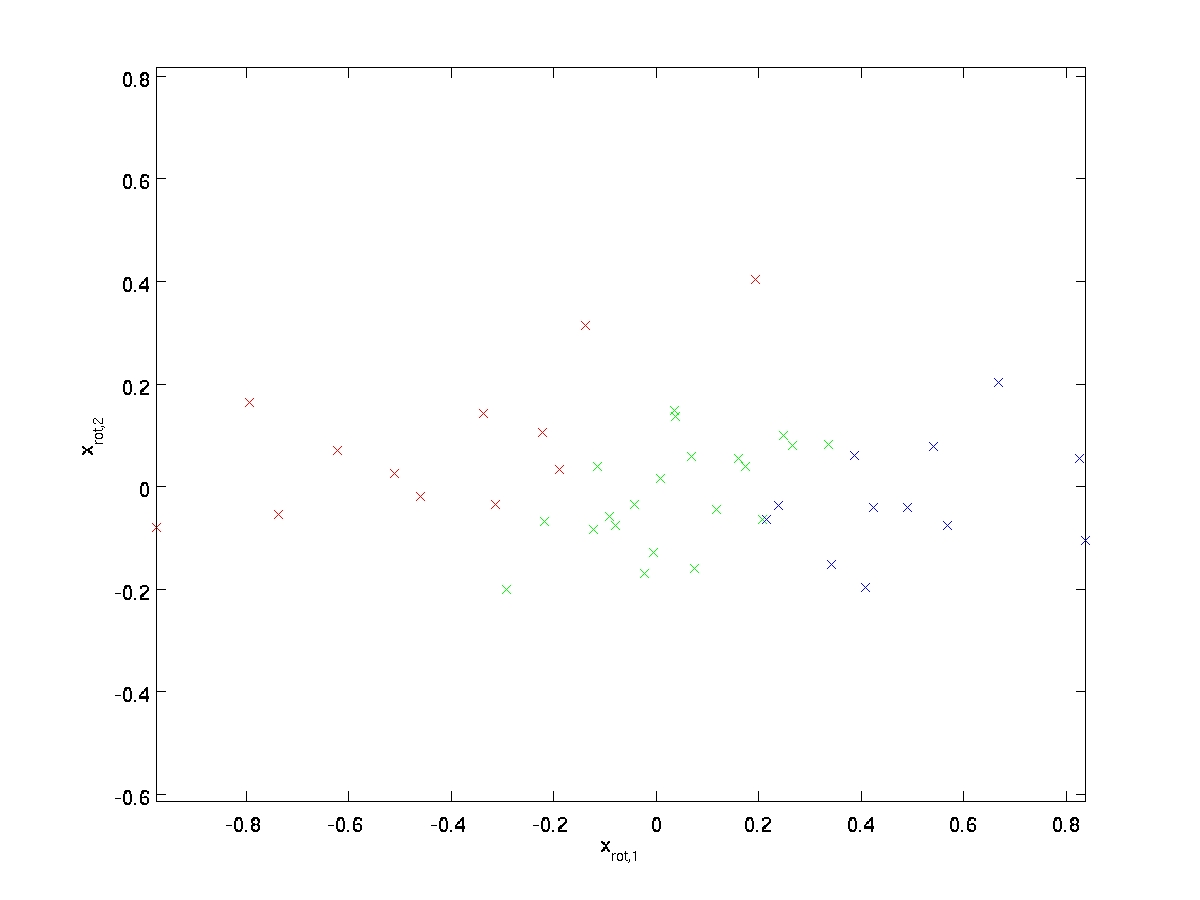
\includegraphics[width=0.8\textwidth]{figures/PCA-rotated.png}
  \caption{}\label{fig:pcarotated}
\end{figure}

\cnt{This is the training set rotated into the $u_1, u_2$ basis. In the general case, $U^Tx$ will be the training set rotated into the basis $u_1, u_2, \ldots, u_n$.}
    {这就是把训练数据集旋转到 $u_1, u_2$ 基后的结果。一般而言,运算 $U^Tx$ 表示旋转到基 $u_1, u_2, \ldots, u_n$ 之上的训练数据。}
    {}

\cnt{One of the properties of $U$ is that it is an ``orthogonal" matrix, which means that it satisfies $U^TU = UU^T = I$. So if you ever need to go from the rotated vectors $x_{\rm rot}$ back to the original data $x$, you can compute}
    {矩阵 $U$ 有正交性,即满足 $U^TU = UU^T = I$,所以若想将旋转后的向量 $x_{\rm rot}$ 还原为原始数据 $x$,将其左乘矩阵$U$ 即可: $x=U x_{\rm rot}$, 验算一下: $U x_{\rm rot} = UU^T x = x$.}
    {}
    \begin{align} x = U x_{\rm rot} , \end{align} 
\cnt{because $U x_{\rm rot} = UU^T x = x$.}
    {}
    {}



\subsubsection{\cnt{Reducing the Data Dimension}{数据降维}{}}

\cnt{We see that the principal direction of variation of the data is the first dimension $x_{{\rm rot},1}$ of this rotated data. Thus, if we want to reduce this data to one dimension, we can set}
    {数据的主方向就是旋转数据的第一维 $x_{{\rm rot},1}$。因此,若想把这数据降到一维,可令:}
    {}
\begin{align} \tilde{x}^{(i)} = x_{{\rm rot},1}^{(i)} = u_1^Tx^{(i)} \in \Re. \end{align}

\cnt{More generally, if $x \in \Re^n$ and we want to reduce it to a $k$ dimensional representation $\tilde{x} \in \Re^k$ (where $k < n$), we would take the first $k$ components of $x_{\rm rot}$, which correspond to the top $k$ directions of variation.}
    {更一般的,假如想把数据 $x \in \Re^n$ 降到 $k$ 维表示 $\tilde{x} \in \Re^k$ (令 $k < n$),只需选取 $x_{\rm rot}$ 的前 $k$ 个成分,分别对应前 $k$ 个数据变化的主方向。}
    {}

\cnt{Another way of explaining PCA is that $x_{\rm rot}$ is an $n$ dimensional vector, where the first few components are likely to be large (e.g., in our example, we saw that $x_{{\rm rot},1}^{(i)} = u_1^Tx^{(i)}$ takes reasonably large values for most examples $i$), and the later components are likely to be small (e.g., in our example, $x_{{\rm rot},2}^{(i)} = u_2^Tx^{(i)}$ was more likely to be small).}
    {PCA的另外一种解释是:$x_{\rm rot}$ 是一个 $n$ 维向量,其中前几个成分可能比较大(例如,上例中大部分样本第一个成分 $x_{{\rm rot},1}^{(i)} = u_1^Tx^{(i)}$ 的取值相对较大),而后面成分可能会比较小(例如,上例中大部分样本的 $x_{{\rm rot},2}^{(i)} = u_2^Tx^{(i)}$ 较小)。}
    {}

\cnt{What PCA does it it drops the the later (smaller) components of $x_{\rm rot}$, and just approximates them with 0's. Concretely, our definition of $\tilde{x}$ can also be arrived at by using an approximation to $x_{{\rm rot}}$ where all but the first $k$ components are zeros. In other words, we have:}
    {PCA算法做的其实就是丢弃 $x_{\rm rot}$ 中后面(取值较小)的成分,就是将这些成分的值近似为零。具体的说,设 $\tilde{x}$ 是 $x_{{\rm rot}}$ 的近似表示,那么将 $x_{{\rm rot}}$ 除了前 $k$ 个成分外,其余全赋值为零,就得到:}
    {}

\begin{align} \tilde{x} = \begin{bmatrix} x_{{\rm rot},1} \\ \vdots \\ x_{{\rm rot},k} \\ 0 \\ \vdots \\ 0 \\ \end{bmatrix} \approx \begin{bmatrix} x_{{\rm rot},1} \\ \vdots \\ x_{{\rm rot},k} \\ x_{{\rm rot},k+1} \\ \vdots \\ x_{{\rm rot},n} \end{bmatrix} = x_{\rm rot} \end{align}

\cnt{In our example, this gives us the following plot of $\tilde{x}$ (using $n=2, k=1$):}
    {在本例中,可得 $\tilde{x}$ 的点图如下(取 $n=2, k=1$ ):}
    {}

\begin{figure}[ht] \centering
  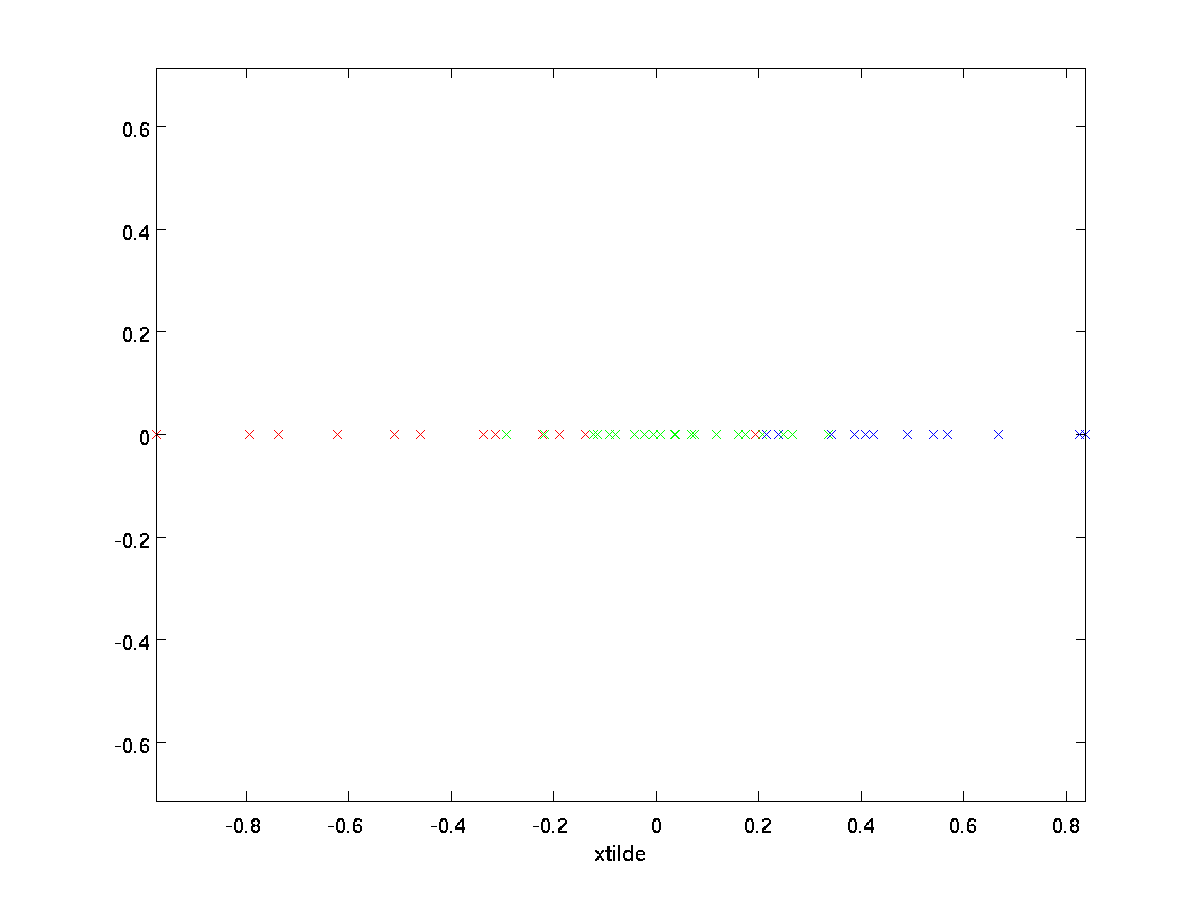
\includegraphics[width=0.8\textwidth]{figures/PCA-xtilde.png}
  %\caption{}\label{fig:step1}
\end{figure}

\cnt{However, since the final $n-k$ components of $\tilde{x}$ as defined above would always be zero, there is no need to keep these zeros around, and so we define $\tilde{x}$ as a $k$-dimensional vector with just the first $k$ (non-zero) components.}
    {然而,由于上面 $\tilde{x}$ 的后 $n-k$ 项均为零,没必要把这些零项保留下来。所以,我们仅用前 $k$ 个(非零)成分来定义 $k$ 维向量 $\tilde{x}$。}
    {}

\cnt{This also explains why we wanted to express our data in the $u_1, u_2, \ldots, u_n$ basis: Deciding which components to keep becomes just keeping the top $k$ components. When we do this, we also say that we are ``retaining the top $k$ PCA (or principal) components."}
    {这也解释了我们为什么会以 $u_1, u_2, \ldots, u_n$ 为基来表示数据:要决定保留哪些成分变得很简单,只需取前 $k$ 个成分即可。这时也可以说,我们“保留了前 $k$ 个PCA(主)成分”。}
    {}


\subsubsection{\cnt{Recovering an Approximation of the Data}{还原近似数据}{}}

\cnt{Now, $\tilde{x} \in \Re^k$ is a lower-dimensional, ``compressed" representation of the original $x \in \Re^n$. Given $\tilde{x}$, how can we recover an approximation $\hat{x}$ to the original value of $x$? From an earlier section(\ref{chp:rotatedatapca}), we know that $x = U x_{\rm rot}$. Further, we can think of $\tilde{x}$ as an approximation to $x_{\rm rot}$, where we have set the last $n-k$ components to zeros. Thus, given $\tilde{x} \in \Re^k$, we can pad it out with $n-k$ zeros to get our approximation to $x_{\rm rot} \in \Re^n$. Finally, we pre-multiply by $U$ to get our approximation to $x$. Concretely, we get}
    {现在,我们得到了原始数据 $x \in \Re^n$ 的低维“压缩”表征量 $\tilde{x} \in \Re^k$, 反过来,如果给定 $\tilde{x}$,我们应如何还原原始数据 $x$ 呢?查看以往章节(\ref{chp:rotatedatapca})可知,要转换回来,只需 $x = U x_{\rm rot}$ 即可。进一步,我们把 $\tilde{x}$ 看作将 $x_{\rm rot}$ 的最后 $n-k$ 个元素被置0所得的近似表示,因此如果给定 $\tilde{x} \in \Re^k$,可以通过在其末尾添加 $n-k$ 个0来得到对 $x_{\rm rot} \in \Re^n$ 的近似,最后,左乘 $U$ 便可近似还原出原数据 $x$。具体来说,计算如下:}
    {}
\begin{align} \hat{x} = U \begin{bmatrix} \tilde{x}_1 \\ \vdots \\ \tilde{x}_k \\ 0 \\ \vdots \\ 0 \end{bmatrix} = \sum_{i=1}^k u_i \tilde{x}_i. \end{align}

\cnt{The final equality above comes from the definition of $U$ given earlier(\ref{chp:examplemathbackground}). (In a practical implementation, we wouldn't actually zero pad $\tilde{x}$ and then multiply by $U$, since that would mean multiplying a lot of things by zeros; instead, we'd just multiply $\tilde{x} \in \Re^k$ with the first $k$ columns of $U$ as in the final expression above.) Applying this to our dataset, we get the following plot for $\hat{x}$:}
    {上面的等式基于先前(\ref{chp:examplemathbackground})对 $U$ 的定义。在实现时,我们实际上并不先给 $\tilde{x}$ 填0然后再左乘 $U$,因为这意味着大量的乘0运算。我们可用 $\tilde{x} \in \Re^k$ 来与 $U$ 的前 $k$ 列相乘,即上式中最右项,来达到同样的目的。将该算法应用于本例中的数据集,可得如下关于重构数据 $\hat{x}$ 的点图:}
    {}

\begin{figure}[ht] \centering
  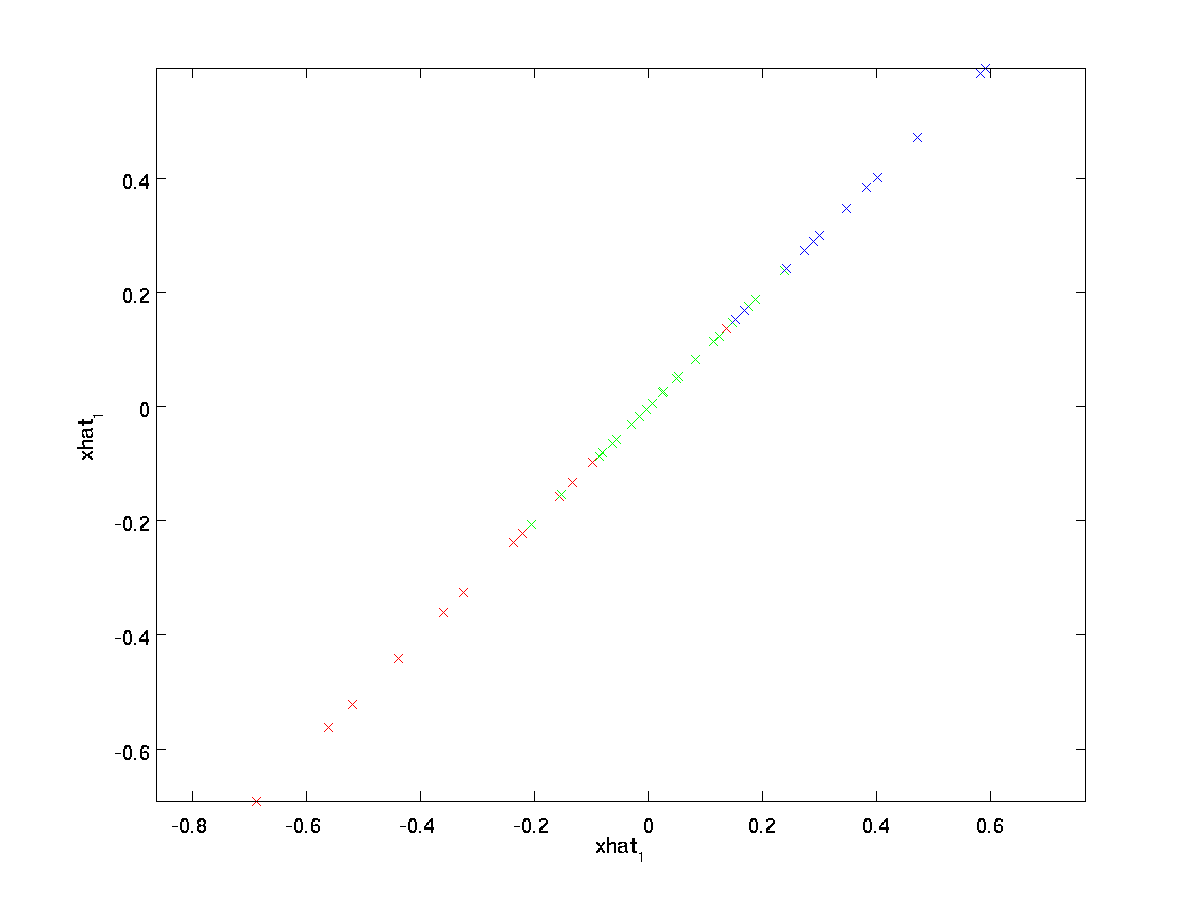
\includegraphics[width=0.8\textwidth]{figures/PCA-xhat.png}
  %\caption{}\label{fig:step1}
\end{figure}

\cnt{We are thus using a 1 dimensional approximation to the original dataset.}
    {由图可见,我们得到的是对原始数据集的一维近似重构。}
    {}

\cnt{If you are training an autoencoder or other unsupervised feature learning algorithm, the running time of your algorithm will depend on the dimension of the input. If you feed $\tilde{x} \in \Re^k$ into your learning algorithm instead of $x$, then you'll be training on a lower-dimensional input, and thus your algorithm might run significantly faster. For many datasets, the lower dimensional $\tilde{x}$ representation can be an extremely good approximation to the original, and using PCA this way can significantly speed up your algorithm while introducing very little approximation error.}
    {在训练自动编码器或其它无监督特征学习算法时,算法运行时间将依赖于输入数据的维数。若用 $\tilde{x} \in \Re^k$ 取代 $x$ 作为输入数据,那么算法就可使用低维数据进行训练,运行速度将显著加快。对于很多数据集来说,低维表征量 $\tilde{x}$ 是原数据集的极佳近似,因此在这些场合使用PCA是很合适的,它引入的近似误差的很小,却可显著地提高你算法的运行速度。}
    {}

\subsubsection{\cnt{Number of components to retain}{选择主成分个数}{}} \label{chp:pcaselectnum}

\cnt{How do we set $k$; i.e., how many PCA components should we retain? In our simple 2 dimensional example, it seemed natural to retain 1 out of the 2 components, but for higher dimensional data, this decision is less trivial. If $k$ is too large, then we won't be compressing the data much; in the limit of $k=n$, then we're just using the original data (but rotated into a different basis). Conversely, if $k$ is too small, then we might be using a very bad approximation to the data.}
    {我们该如何选择 $k$,即保留多少个PCA主成分?在上面这个简单的二维实验中,保留第一个成分看起来是自然的选择。对于高维数据来说,做这个决定就没那么简单:如果 $k$ 过大,数据压缩率不高,在极限情况 $k=n$ 时,等于是在使用原始数据(只是旋转投射到了不同的基);相反地,如果 $k$ 过小,那数据的近似误差太太。}
    {}

\cnt{To decide how to set $k$, we will usually look at the \emph{percentage of variance retained} for different values of $k$. Concretely, if $k=n$, then we have an exact approximation to the data, and we say that 100\% of the variance is retained. I.e., all of the variation of the original data is retained. Conversely, if $k=0$, then we are approximating all the data with the zero vector, and thus 0\% of the variance is retained.}
    {决定 $k$ 值时,我们通常会考虑不同 $k$ 值\emph{可保留的方差百分比}。具体来说,如果 $k=n$,那么我们得到的是对数据的完美近似,也就是保留了100\%的方差,即原始数据的所有变化都被保留下来;相反,如果 $k=0$,那等于是使用零向量来逼近输入数据,也就是只有0\%的方差被保留下来。}
    {}


\cnt{More generally, let $\lambda_1, \lambda_2, \ldots, \lambda_n$ be the eigenvalues of $\Sigma$ (sorted in decreasing order), so that $\lambda_j$ is the eigenvalue corresponding to the eigenvector $u_j$. Then if we retain $k$ principal components, the percentage of variance retained is given by:}
    {一般而言,设 $\lambda_1, \lambda_2, \ldots, \lambda_n$ 表示 $\Sigma$ 的特征值(按由大到小顺序排列),使得 $\lambda_j$ 为对应于特征向量 $u_j$ 的特征值。那么如果我们保留前 $k$ 个成分,则保留的方差百分比可计算为:}
    {}
\begin{align} \frac{\sum_{j=1}^k \lambda_j}{\sum_{j=1}^n \lambda_j}. \end{align}


\cnt{In our simple 2D example above, $\lambda_1 = 7.29$, and $\lambda_2 = 0.69$. Thus, by keeping only $k=1$ principal components, we retained $7.29/(7.29+0.69) = 0.913$, or 91.3\% of the variance.}
    {在上面简单的二维实验中,$\lambda_1 = 7.29, \lambda_2 = 0.69$。因此,如果保留 $k=1$ 个主成分,等于我们保留了 $7.29/(7.29+0.69) = 0.913$,即91.3\%的方差。}
    {}

\cnt{A more formal definition of percentage of variance retained is beyond the scope of these notes. However, it is possible to show that $\lambda_j = \sum_{i=1}^m x_{{\rm rot},j}^2$. Thus, if $\lambda_j \approx 0$, that shows that $x_{{\rm rot},j}$ is usually near 0 anyway, and we lose relatively little by approximating it with a constant 0. This also explains why we retain the top principal components (corresponding to the larger values of $\lambda_j$) instead of the bottom ones. The top principal components $x_{{\rm rot},j}$ are the ones that're more variable and that take on larger values, and for which we would incur a greater approximation error if we were to set them to zero.}
    {对保留方差的百分比进行更正式的定义已超出了本教程的范围,但很容易证明,$\lambda_j = \sum_{i=1}^m x_{{\rm rot},j}^2$ 。因此,如果 $\lambda_j \approx 0$,则说明 $x_{{\rm rot},j}$ 也就基本上接近于0,所以用0来近似它并不会产生多大损失。这也解释了为什么要保留前面的主成分(对应的 $\lambda_j$ 值较大)而不是末尾的那些。 这些前面的主成分 $x_{{\rm rot},j}$ 变化性更大,取值也更大,如果将其设为0势必引入较大的近似误差。}
    {}

\cnt{In the case of images, one common heuristic is to choose $k$ so as to retain 99\% of the variance. In other words, we pick the smallest value of $k$ that satisfies}
    {以处理图像数据为例,一个惯常的经验法则是选择 $k$ 以保留99\%的方差,换句话说,我们选取满足以下条件的最小 $k$ 值:}
    {}
\begin{align} \frac{\sum_{j=1}^k \lambda_j}{\sum_{j=1}^n \lambda_j} \geq 0.99. \end{align}

\cnt{Depending on the application, if you are willing to incur some additional error, values in the 90-98\% range are also sometimes used. When you describe to others how you applied PCA, saying that you chose $k$ to retain 95\% of the variance will also be a much more easily interpretable description than saying that you retained 120 (or whatever other number of) components.}
    {对其它应用,如不介意引入稍大的误差,有时也保留90-98\%的方差范围。若向他人介绍PCA算法详情,告诉他们你选择的 $k$ 保留了95\%的方差,比告诉他们你保留了前120个(或任意某个数字)主成分更好理解。 }
    {}

\subsubsection{\cnt{PCA on Images}{对图像数据应用PCA算法}{}}

\cnt{For PCA to work, usually we want each of the features $x_1, x_2, \ldots, x_n$ to have a similar range of values to the others (and to have a mean close to zero). If you've used PCA on other applications before, you may therefore have separately pre-processed each feature to have zero mean and unit variance, by separately estimating the mean and variance of each feature $x_j$. However, this isn't the pre-processing that we will apply to most types of images. Specifically, suppose we are training our algorithm on natural images, so that $x_j$ is the value of pixel $j$. By ``natural images," we informally mean the type of image that a typical animal or person might see over their lifetime.}
    {为使PCA算法能有效工作,通常我们希望所有的特征 $x_1, x_2, \ldots, x_n$ 都有相似的取值范围(并且均值接近于0)。如果你曾在其它应用中使用过PCA算法,你可能知道有必要单独对每个特征做预处理,即通过估算每个特征 $x_j$ 的均值和方差,而后将其取值范围规整化为零均值和单位方差。但是,对于大部分图像类型,我们却不需要进行这样的预处理。假定我们将在自然图像上训练算法,此时特征 $x_j$ 代表的是像素 $j$ 的值。所谓“自然图像”,不严格的说,是指人或动物在他们一生中所见的那种图像。}
    {}

\cnt{Note: Usually we use images of outdoor scenes with grass, trees, etc., and cut out small (say $16 \times 16$) image patches randomly from these to train the algorithm. But in practice most feature learning algorithms are extremely robust to the exact type of image it is trained on, so most images taken with a normal camera, so long as they aren't excessively blurry or have strange artifacts, should work.}
    {注:通常我们选取含草木等内容的户外场景图片,然后从中随机截取小图像块(如$16 \times 16$像素)来训练算法。在实践中我们发现,大多数特征学习算法对训练图片的确切类型并不敏感,所以大多数用普通照相机拍摄的图片,只要不是特别的模糊或带有非常奇怪的人工痕迹,都可以使用。}
    {}

\cnt{When training on natural images, it makes little sense to estimate a separate mean and variance for each pixel, because the statistics in one part of the image should (theoretically) be the same as any other. This property of images is called \emph{stationarity}.}
    {在自然图像上进行训练时,对每一个像素单独估计均值和方差意义不大,因为(理论上)图像任一部分的统计性质都应该和其它部分相同,图像的这种特性被称作\emph{平稳性}(stationarity)。}
    {}

\cnt{In detail, in order for PCA to work well, informally we require that (i) The features have approximately zero mean, and (ii) The different features have similar variances to each other. With natural images, (ii) is already satisfied even without variance normalization, and so we won't perform any variance normalization. (If you are training on audio data---say, on spectrograms---or on text data---say, bag-of-word vectors---we will usually not perform variance normalization either.) In fact, PCA is invariant to the scaling of the data, and will return the same eigenvectors regardless of the scaling of the input. More formally, if you multiply each feature vector $x$ by some positive number (thus scaling every feature in every training example by the same number), PCA's output eigenvectors will not change.}
    {具体而言,为使PCA算法正常工作,我们通常需要满足以下要求:(1)特征的均值大致为0;(2)不同特征的方差值彼此相似。对于自然图片,即使不进行方差归一化操作,条件(2)也自然满足,故而我们不再进行任何方差归一化操作(对音频数据,如声谱,或文本数据,如词袋向量,我们通常也不进行方差归一化)。实际上,PCA算法对输入数据具有缩放不变性,无论输入数据的值被如何放大(或缩小),返回的特征向量都不改变。更正式的说:如果将每个特征向量 $x$ 都乘以某个正数(即所有特征量被放大或缩小相同的倍数),PCA的输出特征向量都将不会发生变化。}
    {}

\cnt{So, we won't use variance normalization. The only normalization we need to perform then is mean normalization, to ensure that the features have a mean around zero. Depending on the application, very often we are not interested in how bright the overall input image is. For example, in object recognition tasks, the overall brightness of the image doesn't affect what objects there are in the image. More formally, we are not interested in the mean intensity value of an image patch; thus, we can subtract out this value, as a form of mean normalization.}
    {既然我们不做方差归一化,唯一还需进行的规整化操作就是均值规整化,其目的是保证所有特征的均值都在0附近。根据应用,在大多数情况下,我们并不关注所输入图像的整体明亮程度。比如在对象识别任务中,图像的整体明亮程度并不会影响图像中存在的是什么物体。更为正式地说,我们对图像块的平均亮度值不感兴趣,所以可以减去这个值来进行均值规整化。}
    {}

\cnt{Concretely, if $x^{(i)} \in \Re^{n}$ are the (grayscale) intensity values of a $16 \times 16$ image patch ($n=256$), we might normalize the intensity of each image $x^{(i)}$ as follows:}
    {具体的步骤是,如果 $x^{(i)} \in \Re^{n}$ 代表$16 \times 16$的图像块的亮度(灰度)值( $n=256$ ),可用如下算法来对每幅图像进行零均值化操作:}
    {}
$$
\mu^{(i)} := \frac{1}{n} \sum_{j=1}^n x^{(i)}_j
$$
$$
x^{(i)}_j := x^{(i)}_j - \mu^{(i)}, {\rm ~ for all ~} j
$$

\cnt{Note that the two steps above are done separately for each image $x^{(i)}$, and that $\mu^{(i)}$ here is the mean intensity of the image $x^{(i)}$. In particular, this is not the same thing as estimating a mean value separately for each pixel $x_j$.}
    {请注意:1)对每个输入图像块 $x^{(i)}$ 都要单独执行上面两个步骤,2)这里的 $\mu^{(i)}$ 是指图像块 $x^{(i)}$ 的平均亮度值。尤其需要注意的是,这和为每个像素 $x_j$ 单独估算均值是两个完全不同的概念。}
    {}

\cnt{If you are training your algorithm on images other than natural images (for example, images of handwritten characters, or images of single isolated objects centered against a white background), other types of normalization might be worth considering, and the best choice may be application dependent. But when training on natural images, using the per-image mean normalization method as given in the equations above would be a reasonable default.}
    {如果你处理的图像并非自然图像(比如,手写文字,或者白背景正中摆放单独物体),其他规整化操作就值得考虑了,而哪种做法最合适也取决于具体应用场合。但对自然图像而言,对每幅图像进行上述的零均值规整化,是默认而合理的处理。}
    {}

\subsubsection{\cnt{References}{参考文献}{}}
\url{http://cs229.stanford.edu/}




\subsection{\cnt{Whitening}{白化}{}} \label{chp:whitening}

\subsubsection{\cnt{Introduction}{介绍}{}}

\cnt{We have used PCA to reduce the dimension of the data. There is a closely related preprocessing step called \emph{whitening} (or, in some other literatures, \emph{sphering}) which is needed for some algorithms. If we are training on images, the raw input is redundant, since adjacent pixel values are highly correlated. The goal of whitening is to make the input less redundant; more formally, our desiderata are that our learning algorithms sees a training input where (i) the features are less correlated with each other, and (ii) the features all have the same variance.}
    {我们已经了解了如何使用PCA降低数据维度。在一些算法中还需要一个与之相关的预处理步骤,这个预处理过程称为\emph{白化}(一些文献中也叫 \emph{sphering})。举例来说,假设训练数据是图像,由于图像中相邻像素之间具有很强的相关性,所以用于训练时输入是冗余的。白化的目的就是降低输入的冗余性;更正式的说,我们希望通过白化过程使得学习算法的输入具有如下性质:(i)特征之间相关性较低;(ii)所有特征具有相同的方差。}
    {}

\subsubsection{\cnt{2D example}{2D 的例子}{}}

\cnt{We will first describe whitening using our previous 2D example. We will then describe how this can be combined with smoothing, and finally how to combine this with PCA.}
    {下面我们先用前文的2D例子描述白化的主要思想,然后分别介绍如何将白化与平滑和PCA相结合。}
    {}

\cnt{How can we make our input features uncorrelated with each other? We had already done this when computing $x_{\rm rot}^{(i)} = U^Tx^{(i)}$. Repeating our previous figure, our plot for $x_{\rm rot}$ was: }
    {如何消除输入特征之间的相关性? 在前文计算 $x_{\rm rot}^{(i)} = U^Tx^{(i)}$ 时实际上已经消除了输入特征$x^{(i)}$之间的相关性。得到的新特征 $x_{\rm rot}$ 的分布如 图 \ref{fig:pcarotated} 所示:}
    {}

\begin{figure}[ht] \centering
  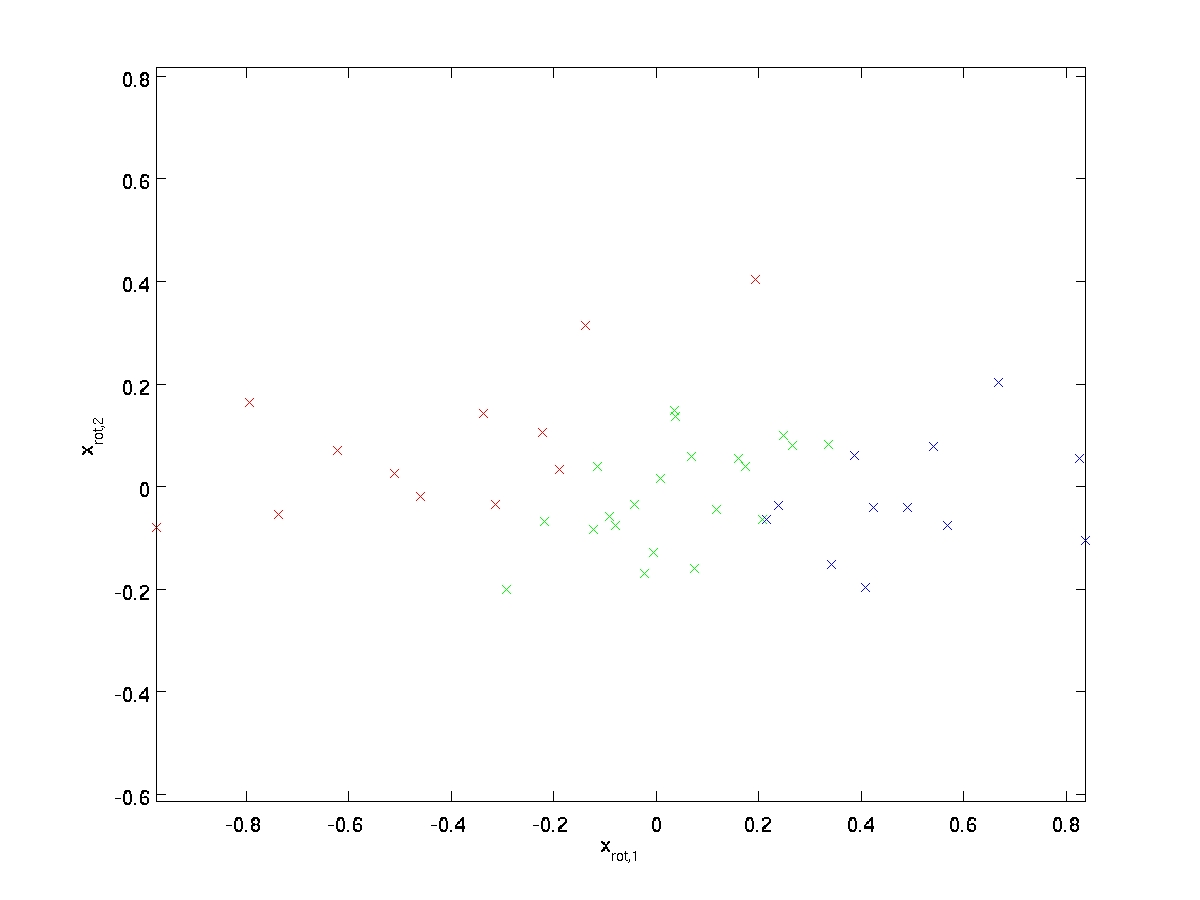
\includegraphics[width=0.8\textwidth]{figures/PCA-rotated.png}
  \caption{}\label{fig:pcarotated2}
\end{figure}

\cnt{The covariance matrix of this data is given by:}
    {这个数据的协方差矩阵如下:}
    {}
\begin{align} \begin{bmatrix} 7.29 & 0 \\ 0 & 0.69 \end{bmatrix}. \end{align}

\cnt{(Note: Technically, many of the statements in this section about the ``covariance" will be true only if the data has zero mean. In the rest of this section, we will take this assumption as implicit in our statements. However, even if the data's mean isn't exactly zero, the intuitions we're presenting here still hold true, and so this isn't something that you should worry about.)}
    {(注: 严格地讲, 这部分许多关于“协方差”的陈述仅当数据均值为0时成立。下文的论述都隐式地假定这一条件成立。不过即使数据均值不为0,下文的说法仍然成立,所以你无需担心这个。)}
    {}

\cnt{It is no accident that the diagonal values are $\lambda_1$ and $\lambda_2$. Further, the off-diagonal entries are zero; thus, $x_{{\rm rot},1}$ and $x_{{\rm rot},2}$ are uncorrelated, satisfying one of our desiderata for whitened data (that the features be less correlated).}
    {$x_{\rm rot}$ 协方差矩阵对角元素的值为 $\lambda_1$ 和 $\lambda_2$ 绝非偶然。并且非对角元素值为0; 因此, $x_{{\rm rot},1}$ 和 $x_{{\rm rot},2}$ 是不相关的, 满足我们对白化结果的第一个要求 (特征间相关性降低)。}
    {}

\cnt{To make each of our input features have unit variance, we can simply rescale each feature $x_{{\rm rot},i}$ by $1/\sqrt{\lambda_i}$. Concretely, we define our whitened data $x_{{\rm PCAwhite}} \in \Re^n$ as follows:}
    {为了使每个输入特征具有单位方差,我们可以直接使用 $1/\sqrt{\lambda_i}$ 作为缩放因子来缩放每个特征 $x_{{\rm rot},i}$。具体地,我们定义白化后的数据 $x_{{\rm PCAwhite}} \in \Re^n$ 如下:}
    {}

\begin{align} x_{{\rm PCAwhite},i} = \frac{x_{{\rm rot},i} }{\sqrt{\lambda_i}}. \end{align}

\cnt{Plotting $x_{{\rm PCAwhite}}$, we get:}
    {绘制出 $x_{{\rm PCAwhite}}$,我们得到:}
    {}

\begin{figure}[ht] \centering
  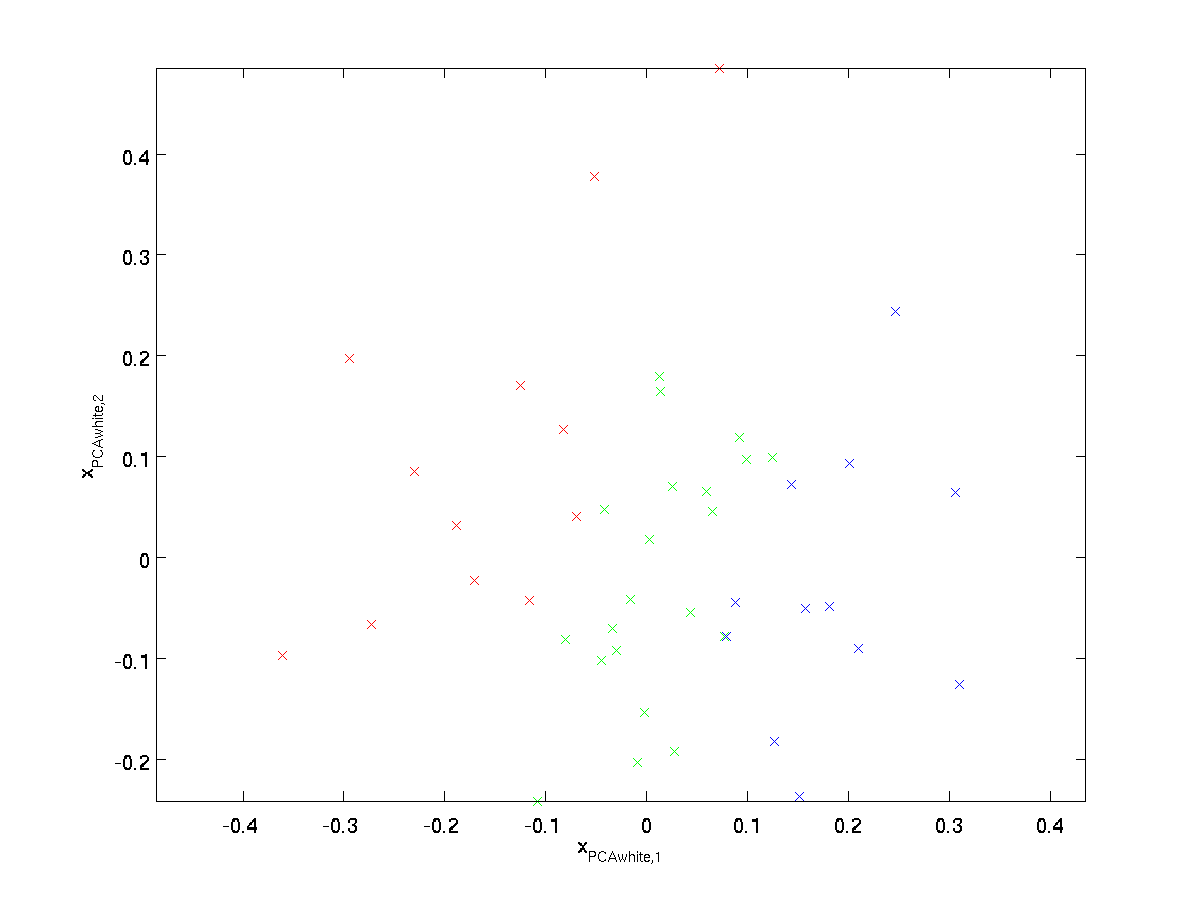
\includegraphics[width=0.8\textwidth]{figures/PCA-whitened.png}
  \caption{}\label{fig:pcarotated2}
\end{figure}

\cnt{This data now has covariance equal to the identity matrix $I$. We say that $x_{{\rm PCAwhite}}$ is our \emph{PCA whitened} version of the data: The different components of $x_{{\rm PCAwhite}}$ are uncorrelated and have unit variance.}
    {这些数据现在的协方差矩阵为单位矩阵 $I$。我们说,$x_{{\rm PCAwhite}}$ 是数据经过\emph{PCA白化}后的版本: $x_{{\rm PCAwhite}}$ 中不同的特征之间不相关并且具有单位方差。}
    {}

\cnt{\emph{Whitening combined with dimensionality reduction}. If you want to have data that is whitened and which is lower dimensional than the original input, you can also optionally keep only the top $k$ components of $x_{{\rm PCAwhite}}$. When we combine PCA whitening with regularization (described later), the last few components of $x_{{\rm PCAwhite}}$ will be nearly zero anyway, and thus can safely be dropped.}
    {\emph{白化与降维相结合}。 如果你想要得到经过白化后的数据,并且比初始输入维数更低,可以仅保留 $x_{{\rm PCAwhite}}$ 中前 $k$ 个成分。当我们把PCA白化和正则化结合起来时(在稍后讨论),$x_{{\rm PCAwhite}}$ 中最后的少量成分将总是接近于0,因而舍弃这些成分不会带来很大的问题。}
    {}

\subsubsection{\cnt{ZCA Whitening}{ZCA白化}{}}

\cnt{Finally, it turns out that this way of getting the data to have covariance identity $I$ isn't unique. Concretely, if $R$ is any orthogonal matrix, so that it satisfies $RR^T = R^TR = I$ (less formally, if $R$ is a rotation/reflection matrix), then $R \,x_{\rm PCAwhite}$ will also have identity covariance. In \emph{ZCA whitening}, we choose $R = U$. We define}
    {最后要说明的是,使数据的协方差矩阵变为单位矩阵 $I$ 的方式并不唯一。具体地,如果 $R$ 是任意正交矩阵,即满足 $RR^T = R^TR = I$ (说它正交不太严格,$R$ 可以是旋转或反射矩阵), 那么 $R \,x_{\rm PCAwhite}$ 仍然具有单位协方差。在\emph{ZCA白化}中,令 $R = U$。我们定义ZCA白化的结果为:}
    {}
\begin{align} x_{\rm ZCAwhite} = U x_{\rm PCAwhite} \end{align}

\cnt{Plotting $x_{\rm ZCAwhite}$, we get:}
    {绘制 $x_{\rm ZCAwhite}$,得到:}
    {}
\begin{figure}[ht] \centering
  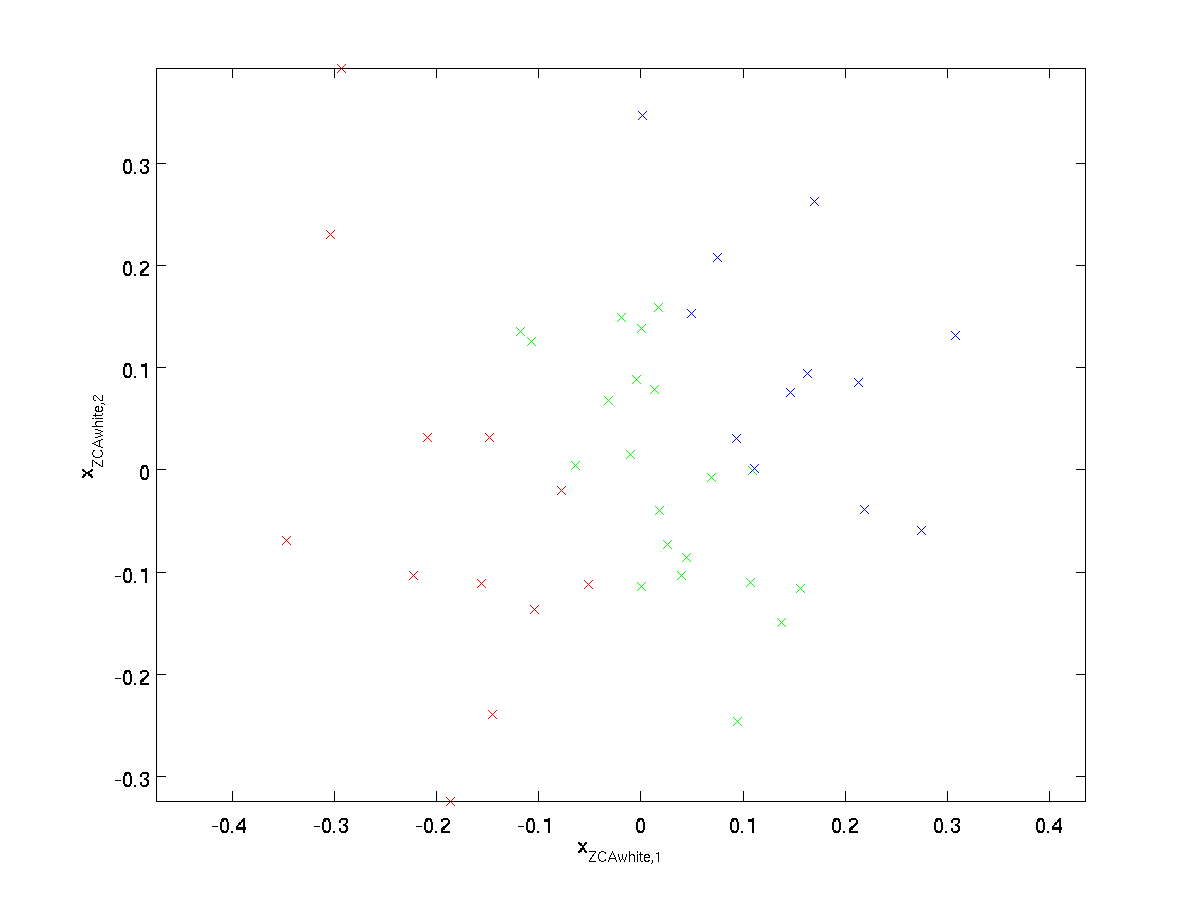
\includegraphics[width=0.8\textwidth]{figures/ZCA-whitened.png}
  %\caption{}\label{fig:zcawhiten}
\end{figure}

\cnt{It can be shown that out of all possible choices for $R$, this choice of rotation causes $x_{\rm ZCAwhite}$ to be as close as possible to the original input data $x$.}
    {可以证明,对所有可能的 $R$,这种旋转使得 $x_{\rm ZCAwhite}$ 尽可能地接近原始输入数据 $x$。}
    {}

\cnt{When using ZCA whitening (unlike PCA whitening), we usually keep all $n$ dimensions of the data, and do not try to reduce its dimension.}
    {当使用 ZCA白化时(不同于 PCA白化),我们通常保留数据的全部 $n$ 个维度,不尝试去降低它的维数。}
    {}

\subsubsection{\cnt{Regularizaton}{正则化}{}}

\cnt{When implementing PCA whitening or ZCA whitening in practice, sometimes some of the eigenvalues $\lambda_i$ will be numerically close to 0, and thus the scaling step where we divide by $\sqrt{\lambda_i}$ would involve dividing by a value close to zero; this may cause the data to blow up (take on large values) or otherwise be numerically unstable. In practice, we therefore implement this scaling step using a small amount of regularization, and add a small constant $\epsilon$ to the eigenvalues before taking their square root and inverse:}
    {实践中需要实现PCA白化或ZCA白化时,有时一些特征值 $\lambda_i$ 在数值上接近于0,这样在缩放步骤时我们除以 $\sqrt{\lambda_i}$ 将导致除以一个接近0的值;这可能使数据上溢 (赋为大数值)或造成数值不稳定。因而在实践中,我们使用少量的正则化实现这个缩放过程,即在取平方根和倒数之前给特征值加上一个很小的常数 $\epsilon$:}
    {}
\begin{align} x_{{\rm PCAwhite},i} = \frac{x_{{\rm rot},i} }{\sqrt{\lambda_i + \epsilon}}. \end{align}

\cnt{When $x$ takes values around $[-1,1]$, a value of $\epsilon \approx 10^{-5}$ might be typical.}
    {当 $x$ 在区间 $[-1,1]$ 上时, 一般取值为 $\epsilon \approx 10^{-5}$。}
    {}

\cnt{For the case of images, adding $\epsilon$ here also has the effect of slightly smoothing (or low-pass filtering) the input image. This also has a desirable effect of removing aliasing artifacts caused by the way pixels are laid out in an image, and can improve the features learned (details are beyond the scope of these notes).}
    {对图像来说, 这里加上 $\epsilon$,对输入图像也有一些平滑(或低通滤波)的作用。这样处理还能消除在图像的像素信息获取过程中产生的噪声,改善学习到的特征(细节超出了本文的范围)。}
    {}

\cnt{ZCA whitening is a form of pre-processing of the data that maps it from $x$ to $x_{\rm ZCAwhite}$. It turns out that this is also a rough model of how the biological eye (the retina) processes images. Specifically, as your eye perceives images, most adjacent ``pixels" in your eye will perceive very similar values, since adjacent parts of an image tend to be highly correlated in intensity. It is thus wasteful for your eye to have to transmit every pixel separately (via your optic nerve) to your brain. Instead, your retina performs a decorrelation operation (this is done via retinal neurons that compute a function called ``on center, off surround/off center, on surround") which is similar to that performed by ZCA. This results in a less redundant representation of the input image, which is then transmitted to your brain.}
    {ZCA 白化是一种数据预处理方法,它将数据从 $x$ 映射到 $x_{\rm ZCAwhite}$。 事实证明这也是一种生物眼睛(视网膜)处理图像的粗糙模型。具体而言,当你的眼睛感知图像时,由于一幅图像中相邻的部分在亮度上十分相关,大多数临近的“像素”在眼中被感知为相近的值。因此,如果人眼需要分别传输每个像素值(通过视觉神经)到大脑中,会非常不划算。取而代之的是,视网膜进行一个与ZCA中相似的去相关操作 (这是由视网膜上的ON-型和OFF-型光感受器细胞将光信号转变为神经信号完成的)。由此得到对输入图像的更低冗余的表示,并将它传输到大脑。}
    {}


\subsection{\cnt{Implementing PCA/Whitening}{实现主成分分析和白化}{}}

\cnt{In this section, we summarize the PCA, PCA whitening and ZCA whitening algorithms, and also describe how you can implement them using efficient linear algebra libraries.}
    {在这一节里,我们将总结PCA, PCA白化和ZCA白化算法,并描述如何使用高效的线性代数库来实现它们。}
    {}

\cnt{First, we need to ensure that the data has (approximately) zero-mean. For natural images, we achieve this (approximately) by subtracting the mean value of each image patch.}
    {首先,我们需要确保数据的均值(近似)为零。对于自然图像,我们通过减去每个图像块(patch)的均值(近似地)来达到这一目标。}
    {}

\cnt{We achieve this by computing the mean for each patch and subtracting it for each patch. In Matlab, we can do this by using}
    {为此,我们计算每个图像块的均值,并从每个图像块中减去它的均值。(译注:参见PCA一章中“对图像数据应用PCA算法”一节)。Matlab实现如下:}
    {}
\begin{lstlisting}[language=matlab]
avg = mean(x, 1);     % Compute the mean pixel intensity value separately for each patch. 
x = x - repmat(avg, size(x, 1), 1);
\end{lstlisting}

\cnt{Next, we need to compute $\Sigma = \frac{1}{m} \sum_{i=1}^m (x^{(i)})(x^{(i)})^T$. If you're implementing this in Matlab (or even if you're implementing this in C++, Java, etc., but have access to an efficient linear algebra library), doing it as an explicit sum is inefficient. Instead, we can compute this in one fell swoop as}
    {下面,我们要计算 $\Sigma = \frac{1}{m} \sum_{i=1}^m (x^{(i)})(x^{(i)})^T$,如果你在Matlab中实现(或者在C++, Java等中实现,但可以使用高效的线性代数库),直接求和效率很低。不过,我们可以这样一气呵成。}
    {}
\begin{lstlisting}[language=matlab]
sigma = x * x' / size(x, 2);
\end{lstlisting}

\cnt{(Check the math yourself for correctness.) Here, we assume that \texttt{x} is a data structure that contains one training example per column (so, \texttt{x} is a $n$-by-$m$ matrix).}
    {(自己推导一下看看)这里,我们假设 \texttt{x} 为一数据结构,其中每列表示一个训练样本(所以 \texttt{x} 是一个 $n \times m$ 的矩阵)。}
    {}

\cnt{Next, PCA computes the eigenvectors of $\Sigma$. One could do this using the Matlab \texttt{eig} function. However, because $\Sigma$ is a symmetric positive semi-definite matrix, it is more numerically reliable to do this using the svd function. Concretely, if you implement}
    {接下来,PCA计算 $\Sigma$ 的特征向量。你可以使用Matlab的 \texttt{eig} 函数来计算。但是由于 $\Sigma$ 是对称半正定的矩阵,用 svd 函数在数值计算上更加稳定。具体来说,如果你使用}
    {}
\begin{lstlisting}[language=matlab]
[U,S,V] = svd(sigma);
\end{lstlisting}
\cnt{then the matrix \texttt{U} will contain the eigenvectors of Sigma (one eigenvector per column, sorted in order from top to bottom eigenvector), and the diagonal entries of the matrix $S$ will contain the corresponding eigenvalues (also sorted in decreasing order). The matrix \texttt{V} will be equal to transpose of \texttt{U}, and can be safely ignored.}
    {那矩阵 \texttt{U} 将包含 Sigma 的特征向量(一个特征向量一列,从主向量开始排序),矩阵 \texttt{S} 对角线上的元素将包含对应的特征值(同样降序排列)。矩阵 \texttt{V} 等于 \texttt{U} 的转置,可以忽略。}
    {}

\cnt{(Note: The svd function actually computes the singular vectors and singular values of a matrix, which for the special case of a symmetric positive semi-definite matrix---which is all that we're concerned with here---is equal to its eigenvectors and eigenvalues. A full discussion of singular vectors vs. eigenvectors is beyond the scope of these notes.)}
    {(注意 svd 函数实际上计算的是一个矩阵的奇异值和奇异向量,就对称半正定矩阵的特殊情况来说,它们对应于特征值和特征向量,这里我们也只关心这一特例。关于奇异向量和特征向量的详细讨论超出了本文范围。)}
    {}

\cnt{Finally, you can compute $x_{\rm rot}$ and $\tilde{x}$ as follows:}
    {最后,我们可以这样计 算$x_{\rm rot}$ 和 $\tilde{x}$:}
    {}
\begin{lstlisting}[language=matlab]
xRot = U' * x;          % rotated version of the data. 
xTilde = U(:,1:k)' * x; % reduced dimension representation of the data, 
                        % where k is the number of eigenvectors to keep
\end{lstlisting}

\cnt{This gives your PCA representation of the data in terms of $\tilde{x} \in \Re^k$. Incidentally, if \texttt{x} is a $n$-by-$m$ matrix containing all your training data, this is a vectorized implementation, and the expressions above work too for computing $x_{\rm rot}$ and $\tilde{x}$ for your entire training set all in one go. The resulting $x_{\rm rot}$ and $\tilde{x}$ will have one column corresponding to each training example.}
    {这以 $\tilde{x} \in \Re^k$ 的形式给出了数据的PCA表示。顺便说一下,如果 \texttt{x} 是一个包括所有训练数据的 $n \times m$ 矩阵,这也是一种向量化的实现方式,上面的式子可以让你一次对所有的训练样本计算出 $x_{\rm rot}$ 和 $\tilde{x}$。得到的 $x_{\rm rot}$ 和 $\tilde{x}$ 中,每列对应一个训练样本。}
    {}

\cnt{To compute the PCA whitened data $x_{\rm PCAwhite}$, use}
    {为计算PCA白化后的数据 $x_{\rm PCAwhite}$,可以用}
    {}
\begin{lstlisting}[language=matlab]
xPCAwhite = diag(1./sqrt(diag(S) + epsilon)) * U' * x;
\end{lstlisting}

\cnt{Since $S$'s diagonal contains the eigenvalues $\lambda_i$, this turns out to be a compact way of computing $x_{{\rm PCAwhite},i} = \dfrac{x_{{\rm rot},i} }{\sqrt{\lambda_i}}$ simultaneously for all $i$.}
    {因为 $S$ 的对角线包括了特征值 $\lambda_i$,这其实就是同时为所有样本 $i$ 计算 $x_{{\rm PCAwhite},i} = \dfrac{x_{{\rm rot},i} }{\sqrt{\lambda_i}}$ 的简洁表达。}
    {}

\cnt{Finally, you can also compute the ZCA whitened data $x_{\rm ZCAwhite}$ as:}
    {最后,你也可以这样计算ZCA白化后的数据 $x_{\rm ZCAwhite}$:}
    {}
\begin{lstlisting}[language=matlab]
xZCAwhite = U * diag(1./sqrt(diag(S) + epsilon)) * U' * x;
\end{lstlisting}


\subsection{\cnt{Exercise:PCA in 2D}{练习:2D中的PCA}{}}

\cnt{PCA, PCA whitening and ZCA whitening in 2D}
    {}
    {}

\cnt{In this exercise you will implement PCA, PCA whitening and ZCA whitening, as described in the earlier sections of this tutorial, and generate the images shown in the earlier sections yourself. You will build on the starter code that has been provided at \url{http://ufldl.stanford.edu/wiki/resources/pca_2d.zip}. You need only write code at the places indicated by ``YOUR CODE HERE" in the files. The only file you need to modify is \texttt{pca\_2d.m}. Implementing this exercise will make the next exercise significantly easier to understand and complete.}
    {}
    {}


\subsubsection{\cnt{Step 0: Load data}{}{}}

\cnt{The starter code contains code to load 45 2D data points. When plotted using the scatter function, the results should look like the following:}
    {}
    {}

\begin{figure}[ht] \centering
  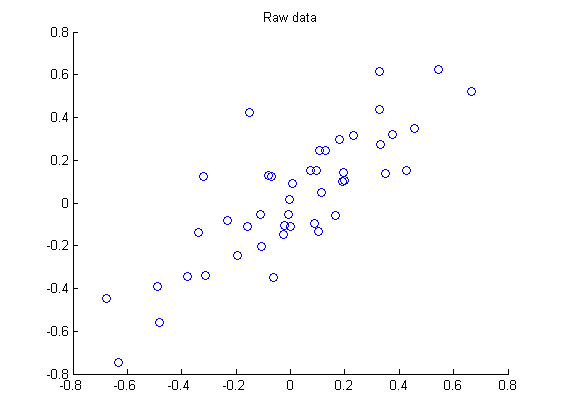
\includegraphics[width=0.8\textwidth]{figures/Raw_images_2d.png}
  %\caption{}\label{fig:zcawhiten}
\end{figure}

\subsubsection{\cnt{Step 1: Implement PCA}{}{}}

\cnt{In this step, you will implement PCA to obtain xrot, the matrix in which the data is ``rotated" to the basis comprising $u_1, \ldots, u_n$ made up of the principal components. As mentioned in the implementation notes, you should make use of MATLAB's svd function here.}
    {}
    {}

\subsubsection{\cnt{Step 1a: Finding the PCA basis}{}{}}

\cnt{Find $u_1$ and $u_2$, and draw two lines in your figure to show the resulting basis on top of the given data points. You may find it useful to use MATLAB's \texttt{hold on} and \texttt{hold off} functions. (After calling \texttt{hold on}, plotting functions such as \texttt{plot} will draw the new data on top of the previously existing figure rather than erasing and replacing it; and \texttt{hold off} turns this off.) You can use \texttt{plot([x1,x2], [y1,y2], '-')} to draw a line between \texttt{(x1,y1)} and \texttt{(x2,y2)}. Your figure should look like this:}
    {}
    {}

\begin{figure}[ht] \centering
  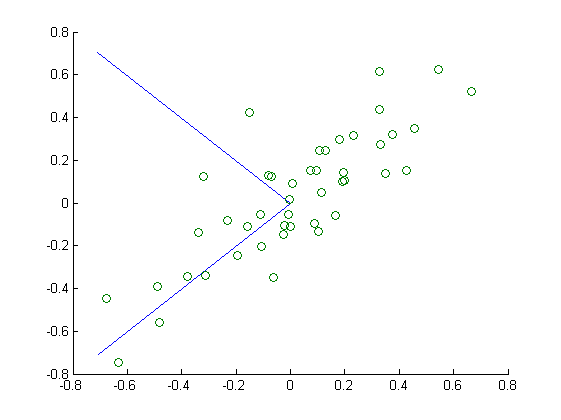
\includegraphics[width=0.8\textwidth]{figures/Pca_2d_basis.png}
  %\caption{}\label{fig:zcawhiten}
\end{figure}


\cnt{If you are doing this in Matlab, you will probably get a plot that's identical to ours. However, eigenvectors are defined only up to a sign. I.e., instead of returning $u_1$ as the first eigenvector, Matlab/Octave could just as easily have returned $-u_1$, and similarly instead of $u_2$ Matlab/Octave could have returned $-u_2$. So if you wound up with one or both of the eigenvectors pointing in a direction opposite (180 degrees difference) from what's shown above, that's okay too.}
    {}
    {}

\subsubsection{\cnt{Step 1b: Check xRot}{}{}}

\cnt{Compute \texttt{xRot}, and use the \texttt{scatter} function to check that \texttt{xRot} looks as it should, which should be something like the following:}
    {}
    {}

\begin{figure}[ht] \centering
  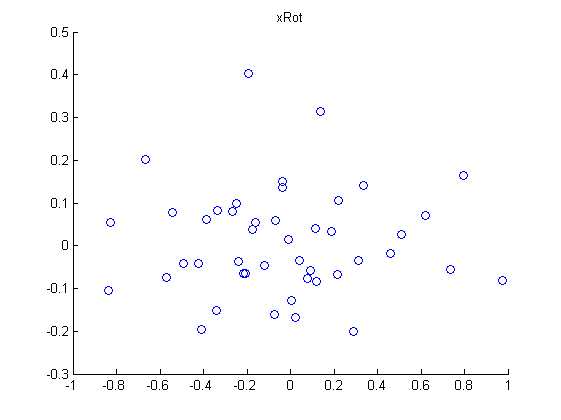
\includegraphics[width=0.8\textwidth]{figures/Pca_xrot_2d.png}
  %\caption{}\label{fig:zcawhiten}
\end{figure}


\cnt{Because Matlab/Octave could have returned $-u_1$ and/or $-u_2$ instead of $u_1$ and $u_2$, it's also possible that you might have gotten a figure which is ``flipped" or ``reflected" along the $x$- and/or $y$-axis; a flipped/reflected version of this figure is also a completely correct result.}
    {}
    {}

\subsubsection{\cnt{Step 2: Dimension reduce and replot}{}{}}

\cnt{In the next step, set $k$, the number of components to retain, to be 1 (we have already done this for you). Compute the resulting xHat and plot the results. You should get the following (this figure should not be flipped along the $x$- or $y$-axis):}
    {}
    {}

\begin{figure}[ht] \centering
  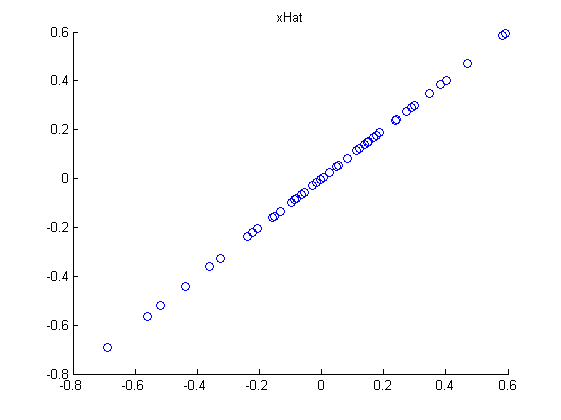
\includegraphics[width=0.8\textwidth]{figures/Pca_xhat_2d.png}
  %\caption{}\label{fig:zcawhiten}
\end{figure}


\subsubsection{\cnt{Step 3: PCA Whitening}{}{}}

\cnt{Implement PCA whitening using the formula from the notes. Plot \texttt{xPCAWhite}, and verify that it looks like the following (a figure that is flipped/reflected on either/both axes is also correct):}
    {}
    {}

\begin{figure}[ht] \centering
  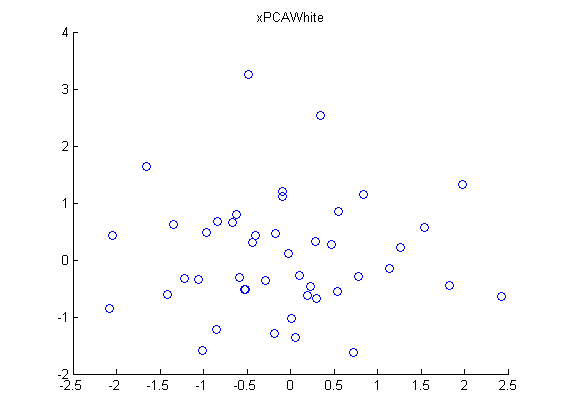
\includegraphics[width=0.8\textwidth]{figures/Pca_white_2d.png}
  %\caption{}\label{fig:zcawhiten}
\end{figure}

\subsubsection{\cnt{Step 4: ZCA Whitening}{}{}}

\cnt{Implement ZCA whitening and plot the results. The results should look like the following (this should not be flipped/reflected along the $x$- or $y$-axis):}
    {}
    {}

\begin{figure}[ht] \centering
  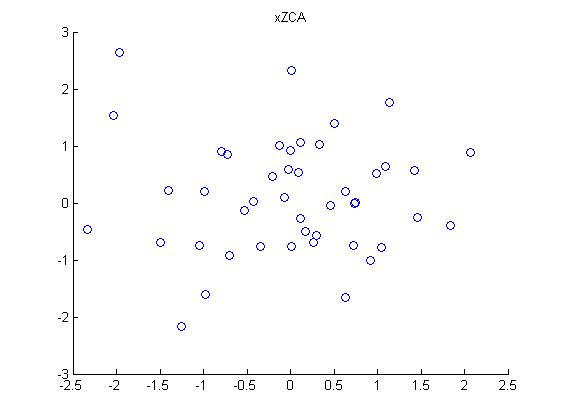
\includegraphics[width=0.8\textwidth]{figures/Zca_white_2d.png}
  %\caption{}\label{fig:zcawhiten}
\end{figure}





\subsection{\cnt{Exercise:PCA and Whitening}{练习:PCA和白化}{}}

\cnt{PCA and Whitening on natural images}
    {}
    {}


\cnt{In this exercise, you will implement PCA, PCA whitening and ZCA whitening, and apply them to image patches taken from natural images.}
    {}
    {}


\cnt{You will build on the MATLAB starter code which we have provided in \url{http://ufldl.stanford.edu/wiki/resources/pca_exercise.zip}{pca\_exercise.zip}. You need only write code at the places indicated by ``YOUR CODE HERE" in the files. The only file you need to modify is \texttt{pca\_gen.m}. }
    {}
    {}

\subsubsection{\cnt{Step 0: Prepare data}{}{}}

\textbf{\cnt{Step 0a: Load data}{}{}}

\cnt{The starter code contains code to load a set of natural images and sample $12 \times 12$ patches from them. The raw patches will look something like this:}
    {}
    {}

\begin{figure}[ht] \centering
  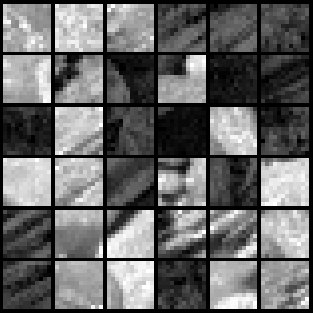
\includegraphics[width=0.5\textwidth]{figures/Raw_images.png}
  %\caption{}\label{fig:zcawhiten}
\end{figure}

\cnt{These patches are stored as column vectors $x^{(i)} \in \mathbb{R}^{144}$ in the $144 \times 10000$ matrix \texttt{x}.}
    {}
    {}

\textbf{\cnt{Step 0b: Zero mean the data}{}{}}

\cnt{First, for each image patch, compute the mean pixel value and subtract it from that image, this centering the image around zero. You should compute a different mean value for each image patch.}
    {}
    {}

\subsubsection{\cnt{Step 1: Implement PCA}{}{}}

\textbf{\cnt{Step 1a: Implement PCA}{}{}}

\cnt{n this step, you will implement PCA to obtain $x_{\rm rot}$, the matrix in which the data is ``rotated" to the basis comprising the principal components (i.e. the eigenvectors of $\Sigma$). Note that in this part of the exercise, you should not whiten the data.}
    {}
    {}

\textbf{\cnt{Step 1b: Check covariance}{}{}}

\cnt{To verify that your implementation of PCA is correct, you should check the covariance matrix for the rotated data $x_{\rm rot}$. PCA guarantees that the covariance matrix for the rotated data is a diagonal matrix (a matrix with non-zero entries only along the main diagonal). Implement code to compute the covariance matrix and verify this property. One way to do this is to compute the covariance matrix, and visualise it using the MATLAB command imagesc. The image should show a coloured diagonal line against a blue background. For this dataset, because of the range of the diagonal entries, the diagonal line may not be apparent, so you might get a figure like the one show below, but this trick of visualizing using imagesc will come in handy later in this exercise.}
    {}
    {}

\begin{figure}[ht] \centering
  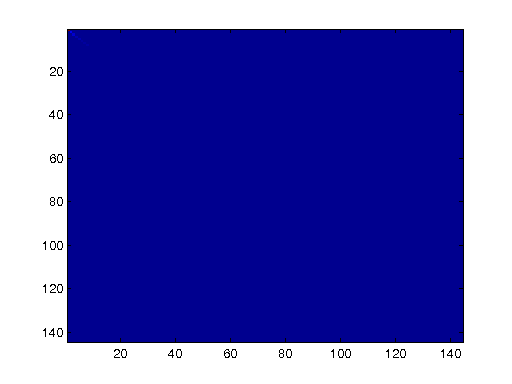
\includegraphics[width=0.4\textwidth]{figures/Pca_covar.png}
  %\caption{}\label{fig:zcawhiten}
\end{figure}

\subsubsection{\cnt{Step 2: Find number of components to retain}{}{}}

\cnt{Next, choose k, the number of principal components to retain. Pick $k$ to be as small as possible, but so that at least 99\% of the variance is retained. In the step after this, you will discard all but the top $k$ principal components, reducing the dimension of the original data to k.}
    {}
    {}

\subsubsection{\cnt{Step 3: PCA with dimension reduction}{}{}}

\cnt{Now that you have found $k$, compute $\tilde{x}$, the reduced-dimension representation of the data. This gives you a representation of each image patch as a $k$ dimensional vector instead of a 144 dimensional vector. If you are training a sparse autoencoder or other algorithm on this reduced-dimensional data, it will run faster than if you were training on the original 144 dimensional data.}
    {}
    {}

\cnt{To see the effect of dimension reduction, go back from $\tilde{x}$ to produce the matrix $\hat{x}$, the dimension-reduced data but expressed in the original 144 dimensional space of image patches. Visualise $\hat{x}$ and compare it to the raw data, $x$. You will observe that there is little loss due to throwing away the principal components that correspond to dimensions with low variation. For comparison, you may also wish to generate and visualise $\hat{x}$ for when only 90\% of the variance is retained.}
    {}
    {}

\begin{figure}[ht] \centering
  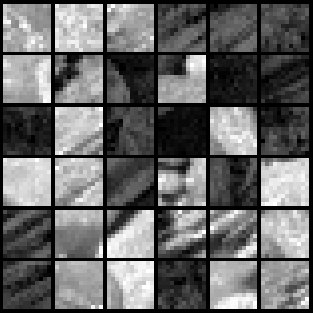
\includegraphics[width=0.3\textwidth]{figures/Raw_images.png} \caption{Raw images}
  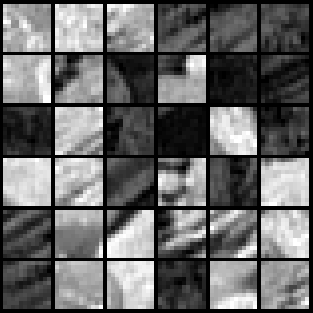
\includegraphics[width=0.3\textwidth]{figures/Pca_images.png} \caption{PCA dimension-reduced images (99\% variance)}
  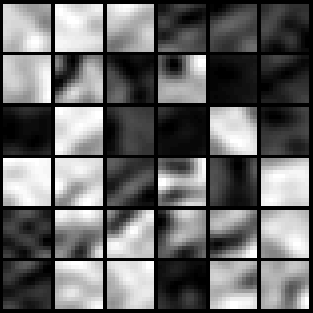
\includegraphics[width=0.3\textwidth]{figures/Pca_images_90.png} \caption{PCA dimension-reduced images (90\% variance)}
  %\caption{}\label{fig:zcawhiten}
\end{figure}

\subsubsection{\cnt{Step 4: PCA with whitening and regularization}{}{}}

\textbf{\cnt{Step 4a: Implement PCA with whitening and regularization}{}{}}

\cnt{Now implement PCA with whitening and regularization to produce the matrix \texttt{xPCAWhite}. Use the following parameter value:}
    {}
    {}
\begin{lstlisting}[language=matlab]
epsilon = 0.1
\end{lstlisting}

\textbf{\cnt{Step 4b: Check covariance}{}{}}

\cnt{Similar to using PCA alone, PCA with whitening also results in processed data that has a diagonal covariance matrix. However, unlike PCA alone, whitening additionally ensures that the diagonal entries are equal to 1, i.e. that the covariance matrix is the identity matrix.}
    {}
    {}

\cnt{That would be the case if you were doing whitening alone with no regularization. However, in this case you are whitening with regularization, to avoid numerical/etc. problems associated with small eigenvalues. As a result of this, some of the diagonal entries of the covariance of your \texttt{xPCAwhite} will be smaller than 1.}
    {}
    {}

\cnt{To verify that your implementation of PCA whitening with and without regularization is correct, you can check these properties. Implement code to compute the covariance matrix and verify this property. (To check the result of PCA without whitening, simply set epsilon to 0, or close to 0, say 1e-10). As earlier, you can visualise the covariance matrix with imagesc. When visualised as an image, for PCA whitening without regularization you should see a red line across the diagonal (corresponding to the one entries) against a blue background (corresponding to the zero entries); for PCA whitening with regularization you should see a red line that slowly turns blue across the diagonal (corresponding to the 1 entries slowly becoming smaller).}
    {}
    {}

\begin{figure}[ht] \centering
  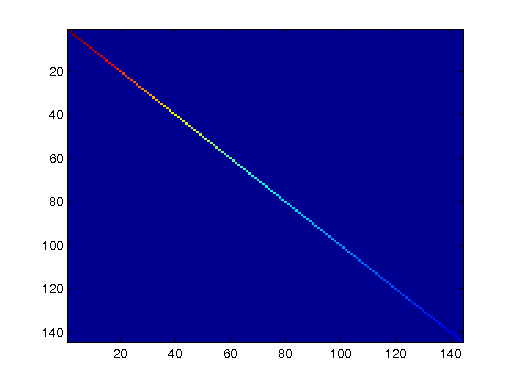
\includegraphics[width=0.4\textwidth]{figures/Pca_whitened_covar.png} \caption{Covariance for PCA whitening with regularization}
  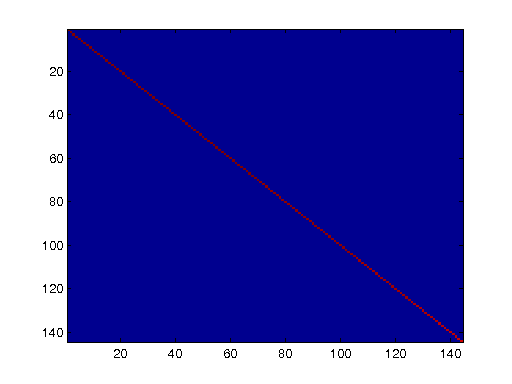
\includegraphics[width=0.4\textwidth]{figures/Pca_whitened_unregularised_covar.png} \caption{Covariance for PCA whitening without regularization}
  %\caption{}\label{fig:zcawhiten}
\end{figure}

\subsubsection{\cnt{Step 5: ZCA whitening}{}{}}

\cnt{Now implement ZCA whitening to produce the matrix \texttt{xZCAWhite}. Visualize \texttt{xZCAWhite} and compare it to the raw data, $x$. You should observe that whitening results in, among other things, enhanced edges. Try repeating this with epsilon set to 1, 0.1, and 0.01, and see what you obtain. The example shown below (left image) was obtained with epsilon = 0.1.}
    {}
    {}

\begin{figure}[ht] \centering
  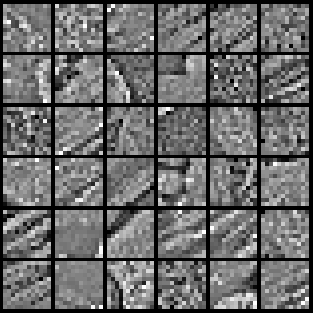
\includegraphics[width=0.4\textwidth]{figures/Zca_whitened_images.png} \caption{ZCA whitened images}
  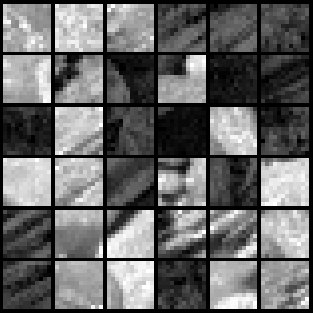
\includegraphics[width=0.4\textwidth]{figures/Raw_images.png} \caption{Raw images}
  %\caption{}\label{fig:zcawhiten}
\end{figure}


